% ==============================================================================
% 第 12 章：综合项目：列表 (Chapter 12: Projects: Lists)
% ==============================================================================

\chapter{综合项目：列表}
\label{sec:ch12_projects}

本章提供了一组综合性项目练习，旨在全面巩固你对程序设计核心要素的理解：批处理与交互式程序设计、基于组合的设计思想、愿望清单管理、以及针对自引用数据的设计配方。

本章首先探讨现实世界的大规模数据处理：英语词典与 iTunes 音乐库；接着通过两个小节剖析单词字谜游戏，展示如何将复杂问题解构为高内聚子任务；随后的章节带领你通过\term{迭代细化}（iterative refinement）开发贪吃蛇、俄罗斯方块、太空大战等经典游戏；最后一节则实现能够解释执行正则表达式与通用有限状态机的模拟引擎。

\section{现实世界的数据：词典}
\label{sec:ch12_dictionaries}

现实世界中的信息往往以极其庞大的规模出现，这正是编写程序处理它们的意义所在。例如，一本英语词典并非包含十几个单词，而是收录数十万个词条。在处理如此大规模的数据时，必须严格遵循设计配方：先在小型输入样例上精心设计并验证函数逻辑，一旦确信无误，再将其投入到真实的真实世界数据中运行。如果程序运行过于缓慢，请反思函数内部是否存在冗余的重复遍历或计算。

\begin{figure}[htbp]
  \centering
  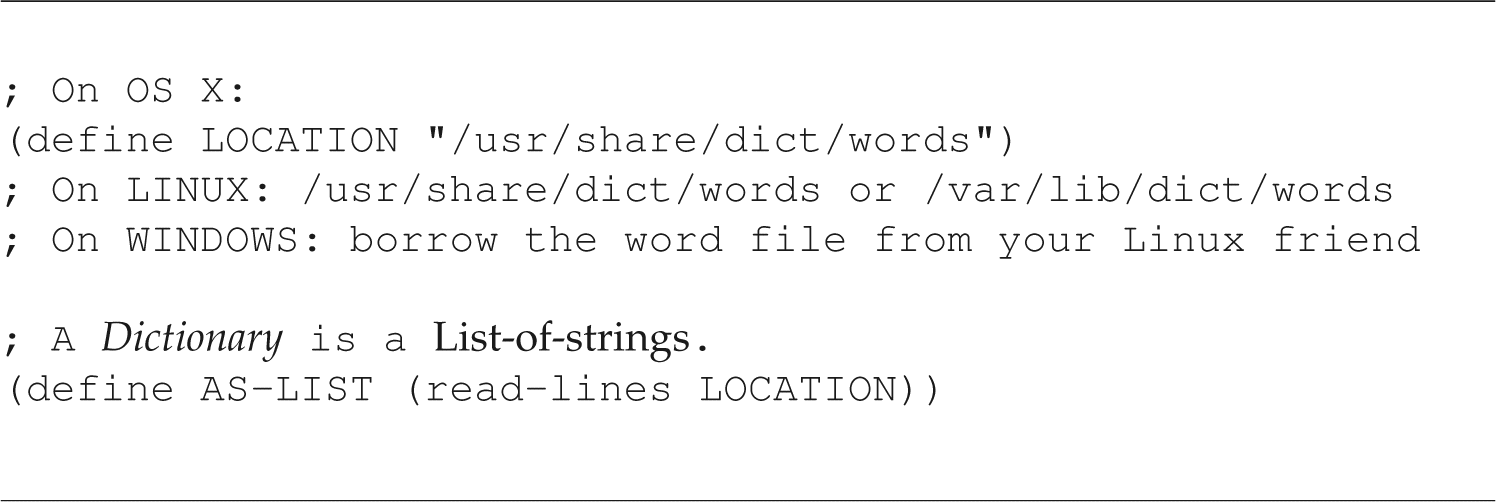
\includegraphics[width=0.85\textwidth]{images/00276.png}
  \caption{从操作系统中读取整本英语词典}
  \label{fig:reading_dictionary}
\end{figure}

在 BSL+ 中，通过 \code{2htdp/batch-io} 库中的 \code{read-words} 函数，只需一行代码即可将系统的整本英语词典加载为一个庞大的字符串列表（如图~\ref{fig:reading_dictionary} 所示）。

在下列练习中，字母扮演着重要角色，我们定义所有英文字母的列表：
\begin{lstlisting}[language=BSL]
; A Letter 是以下单字符 1String 之一：
; -- "a"
; -- ...
; -- "z"
(define LETTERS (explode "abcdefghijklmnopqrstuvwxyz"))
\end{lstlisting}

\begin{exercise}{统计指定字母开头的单词数 starts-with\#}{195}
设计函数 \code{starts-with\#}：接收一个 \code{Letter} 与一个 \code{Dictionary}（单词列表），统计词典中有多少个单词以该指定字母开头。验证函数正确后，统计你的计算机词典中以 \code{"e"} 和以 \code{"z"} 开头的单词数量。
\end{exercise}

\begin{exercise}{全字母词频统计 count-by-letter}{196}
设计结构体与数据定义 \code{Letter-Count}，用于保存一个字母及其对应的词频统计数：
\begin{lstlisting}[language=BSL]
(define-struct lc [letter count])
; A Letter-Count 是一个结构体：(make-lc Letter Number)
\end{lstlisting}
接着设计函数 \code{count-by-letter}：接收一个 \code{Dictionary}，统计 26 个英文字母各自作为单词首字母的出现频率，返回一个 \code{Letter-Count} 列表。
\end{exercise}

\begin{exercise}{寻找最常见首字母 most-frequent}{197}
设计函数 \code{most-frequent}：接收一个 \code{Dictionary}，返回作为首字母出现次数最多的那个 \code{Letter-Count}。你的词典中最频繁出现的首字母是哪一个？它出现了多少次？
\end{exercise}

\begin{exercise}{按首字母分组与中间结构消除（Deforestation 优化）}{198}
设计函数 \code{words-by-first-letter}：接收一个 \code{Dictionary}，产生一个由词典构成的列表（\code{List-of-Dictionary}），每个子词典汇集以某一特定字母开头的单词。

随后利用该函数重构练习 197 中的 \code{most-frequent} 为 \code{most-frequent.v2}，并验证两个版本在真实词典上的输出完全一致。

\begin{notebox}[编程语境：中间数据结构与“森林砍伐” (Deforestation)]
第二种设计方案通过构建庞大的中间分组词典列表来计算最终结果，这些中间数据除了供后续统计之外并无其他作用。在现代高级语言编译器中，有时会自动执行“森林砍伐”（Deforestation，即消除中间数据结构）优化，将两个连续遍历的函数融合为一个，从而消除中间数据结构带来的内存与遍历开销。在未启用此类优化的语言中，如果程序运行缓慢，应考虑避免创建不必要的中间数据结构。
\end{notebox}
\end{exercise}

\section{现实世界的数据：iTunes 播放列表}
\label{sec:ch12_itunes}

苹果公司的 iTunes（以及随后的 Music 应用）能够将其媒体数据库导出为标准的 XML 文件。借助 \code{2htdp/itunes} 教学库，我们能够将音乐曲目导入 BSL 程序进行查询与统计。

在本节中，我们考察两种不同的数据表示法：
\begin{enumerate}
  \item \textbf{基于结构体的表示}（\code{Track} 和 \code{Date}，如图~\ref{fig:itunes_structures} 与图~\ref{fig:itunes_functions} 所示）：每个曲目具有固定的 8 个字段，属性完备、强类型化。
  \item \textbf{基于关联列表的表示}（\code{LLists}，如图~\ref{fig:itunes_lists} 所示）：采用半结构化（semi-structured）键值对列表，允许各曲目包含不同数量的非规范化属性。
\end{enumerate}

\begin{figure}[htbp]
  \centering
  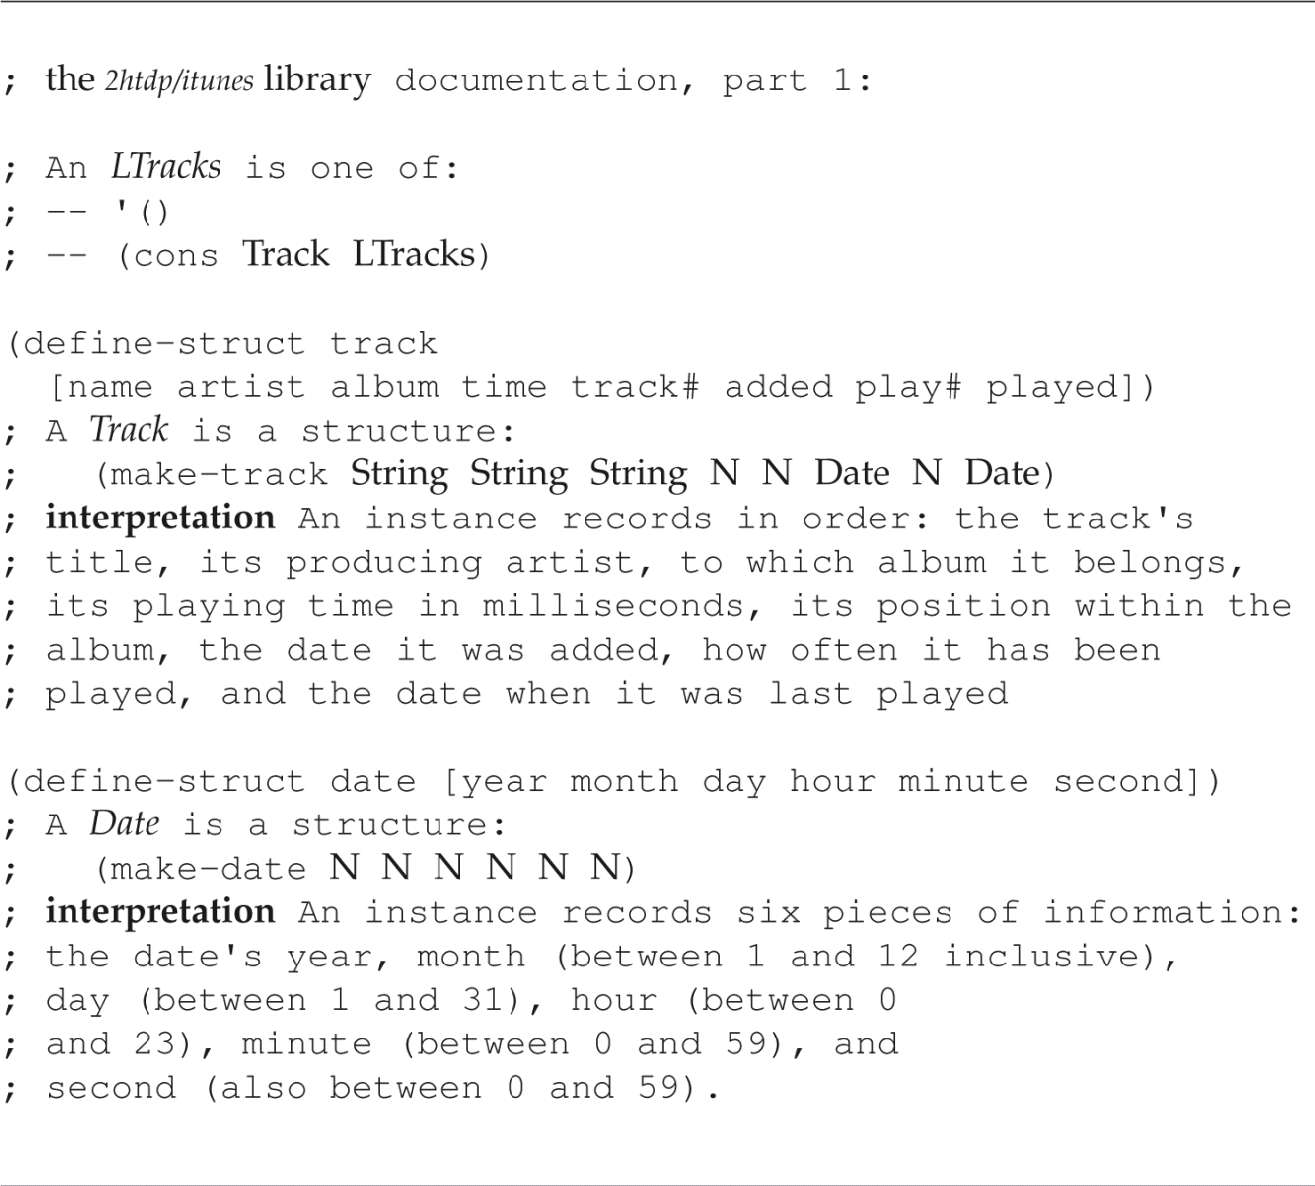
\includegraphics[width=0.85\textwidth]{images/00277.png}
  \caption{基于结构体的 iTunes 曲目数据定义}
  \label{fig:itunes_structures}
\end{figure}

\begin{figure}[htbp]
  \centering
  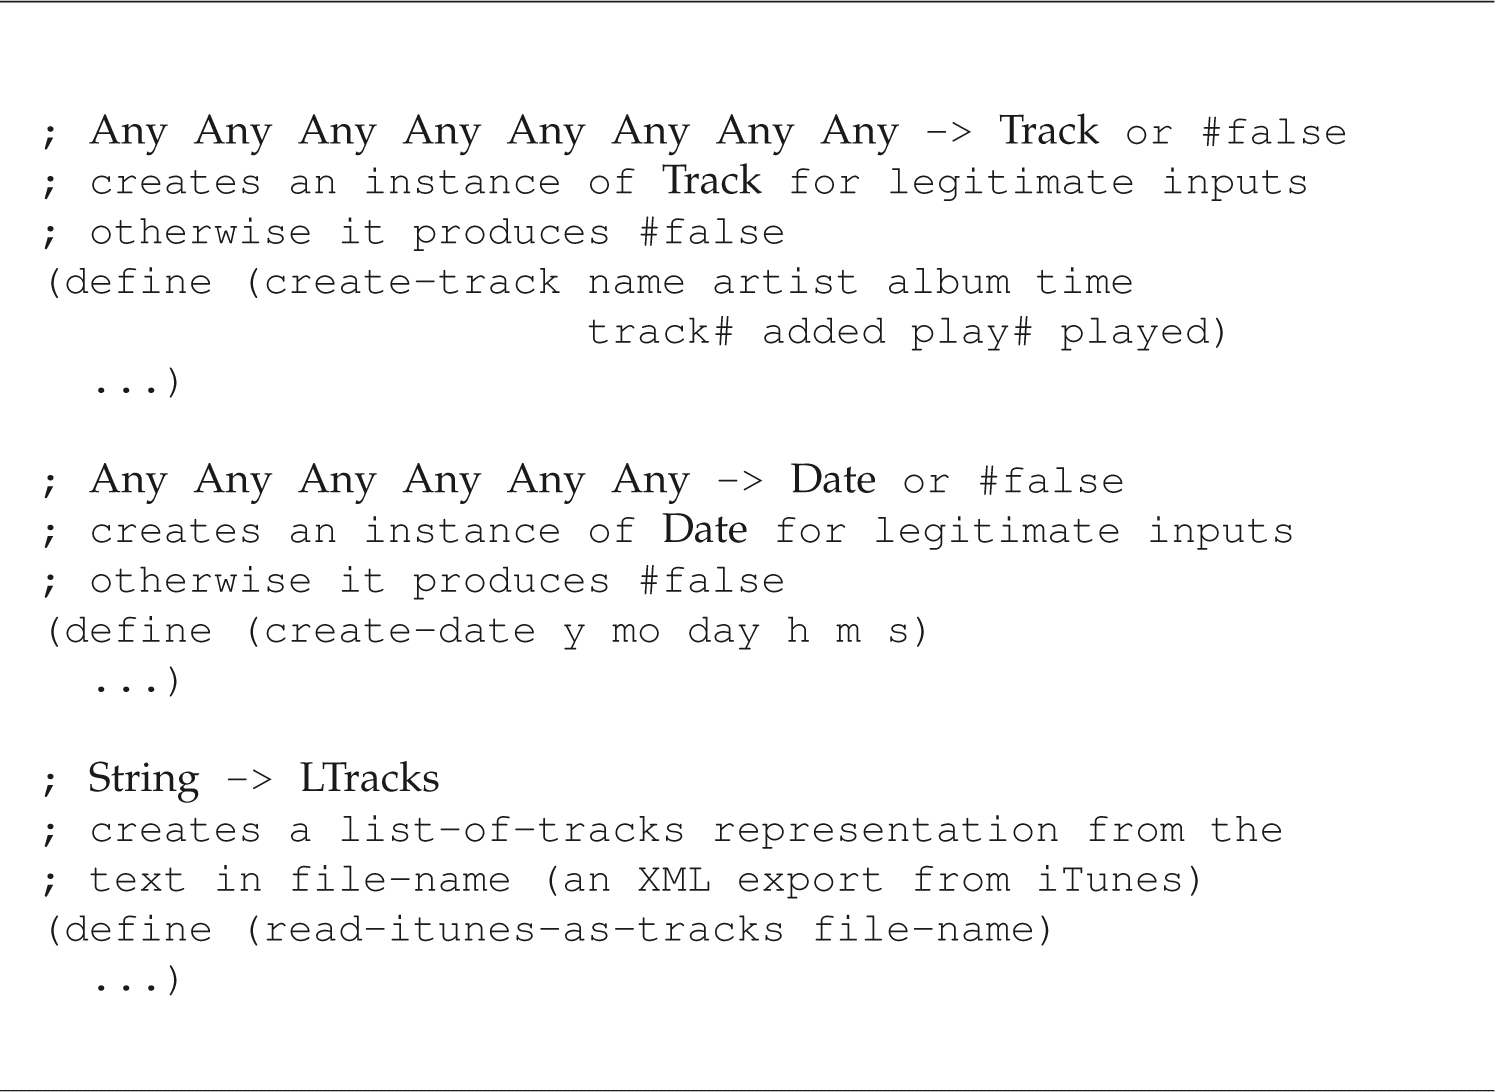
\includegraphics[width=0.85\textwidth]{images/00278.png}
  \caption{iTunes 库函数接口}
  \label{fig:itunes_functions}
\end{figure}

\begin{exercise}{构造曲目示例}{199}
构造若干 \code{Date}、\code{Track} 和 \code{LTracks}（曲目列表）的示例，用于后续测试。
\end{exercise}

\begin{exercise}{累计播放时长 total-time}{200}
设计函数 \code{total-time}：接收一个 \code{LTracks}，计算并返回所有曲目的总播放时间（单位：毫秒）。
\end{exercise}

\begin{exercise}{提取不重复专辑名 select-album-titles/unique}{201}
设计函数 \code{select-all-album-titles}：提取 \code{LTracks} 中的所有专辑名称（可能包含重复项）。

接着设计集合去重函数 \code{create-set}：消耗字符串列表，返回去除了所有重复项的集合列表。

最后组合二者实现 \code{select-album-titles/unique}，输出所有独一无二的专辑名称列表。
\end{exercise}

\begin{exercise}{专辑查询 select-album}{202}
设计函数 \code{select-album}：消耗专辑名称与 \code{LTracks}，提取并返回属于该专辑的所有曲目列表。
\end{exercise}

\begin{exercise}{按日期筛选 select-album-date}{203}
设计函数 \code{select-album-date}：消耗专辑名、指定日期 \code{Date} 以及 \code{LTracks}，筛选出属于该专辑且在指定日期之后播放过的所有曲目。
\end{exercise}

\begin{exercise}{数据库查询：按专辑分组 select-albums}{204}
设计函数 \code{select-albums}：消耗 \code{LTracks}，返回一个由曲目列表构成的列表（\code{List-of-LTracks}），其中每个子列表包含且仅包含属于同一张专辑的所有曲目。
\end{exercise}

\begin{figure}[htbp]
  \centering
  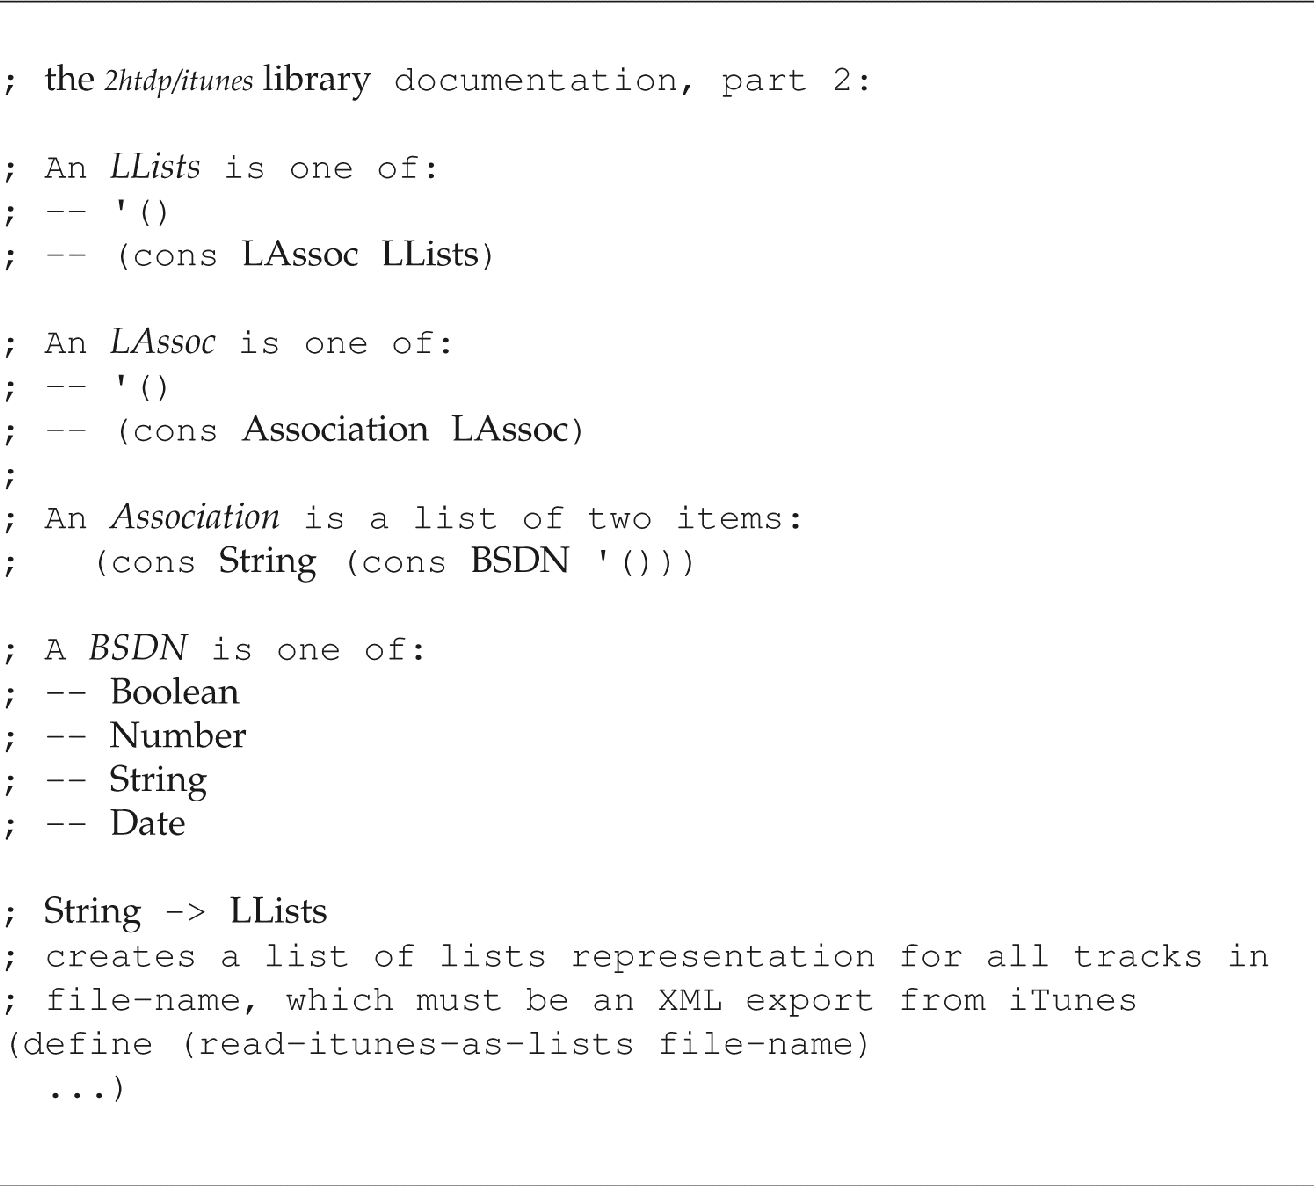
\includegraphics[width=0.85\textwidth]{images/00279.png}
  \caption{基于键值对关联列表的 iTunes 数据表示}
  \label{fig:itunes_lists}
\end{figure}

\begin{exercise}{半结构化曲目示例与查询 find-association}{205}
构造图~\ref{fig:itunes_lists} 中 \code{LAssoc} 与 \code{LLists} 的具体示例。
\end{exercise}

\begin{exercise}{关联查找函数 find-association}{206}
设计函数 \code{find-association}：消耗键名 \code{key}（字符串）、关联列表 \code{LAssoc} 以及默认值 \code{default}。返回首个键名为 \code{key} 的关联项；若未找到，则返回 \code{default}。
\end{exercise}

\begin{exercise}{基于列表表示的播放时长统计}{207}
针对 \code{LLists} 设计 \code{total-time/list} 函数，计算总播放时长。
\end{exercise}

\begin{exercise}{布尔属性提取 boolean-attributes}{208}
设计函数 \code{boolean-attributes}：提取并返回其属性值为布尔类型的所有属性名称列表（去重后）。
\end{exercise}

\section{单词游戏：图解组合设计}
\label{sec:ch12_word_games_composition}

许多人都喜欢字谜游戏。考虑以下例题：
\begin{notebox}[字谜求解]
给定一个英文单词，找出所有由完全相同字母构成的合法英文单词（换位词，Anagram）。例如输入 \code{"cat"}，其字母排列组合还可构成合法词 \code{"act"}。
\end{notebox}

例如对于单词 \code{"dear"}，其 4 个字母共有 $4! = 24$ 种排列方式，其中在词典中合法存在的单词有 3 个：\code{"read"}、\code{"dear"} 和 \code{"dare"}。

人工解决此问题的思路是：先枚举出给定单词中所有字母的所有可能排列组合，然后再逐一查词典，保留那些真正属于词典的单词。这天然指导我们将程序分解为若干函数的串联组合：
\begin{lstlisting}[language=BSL]
; String -> List-of-strings
; 查找由 s 的所有字母构成的所有同字母异序词
(define (alternative-words s)
  (in-dictionary
    (words->strings
      (arrangements (string->word s)))))
\end{lstlisting}

图~\ref{fig:finding_alternative_words} 展示了这一高层组合设计的架构与各函数的职责划分。

\begin{figure}[htbp]
  \centering
  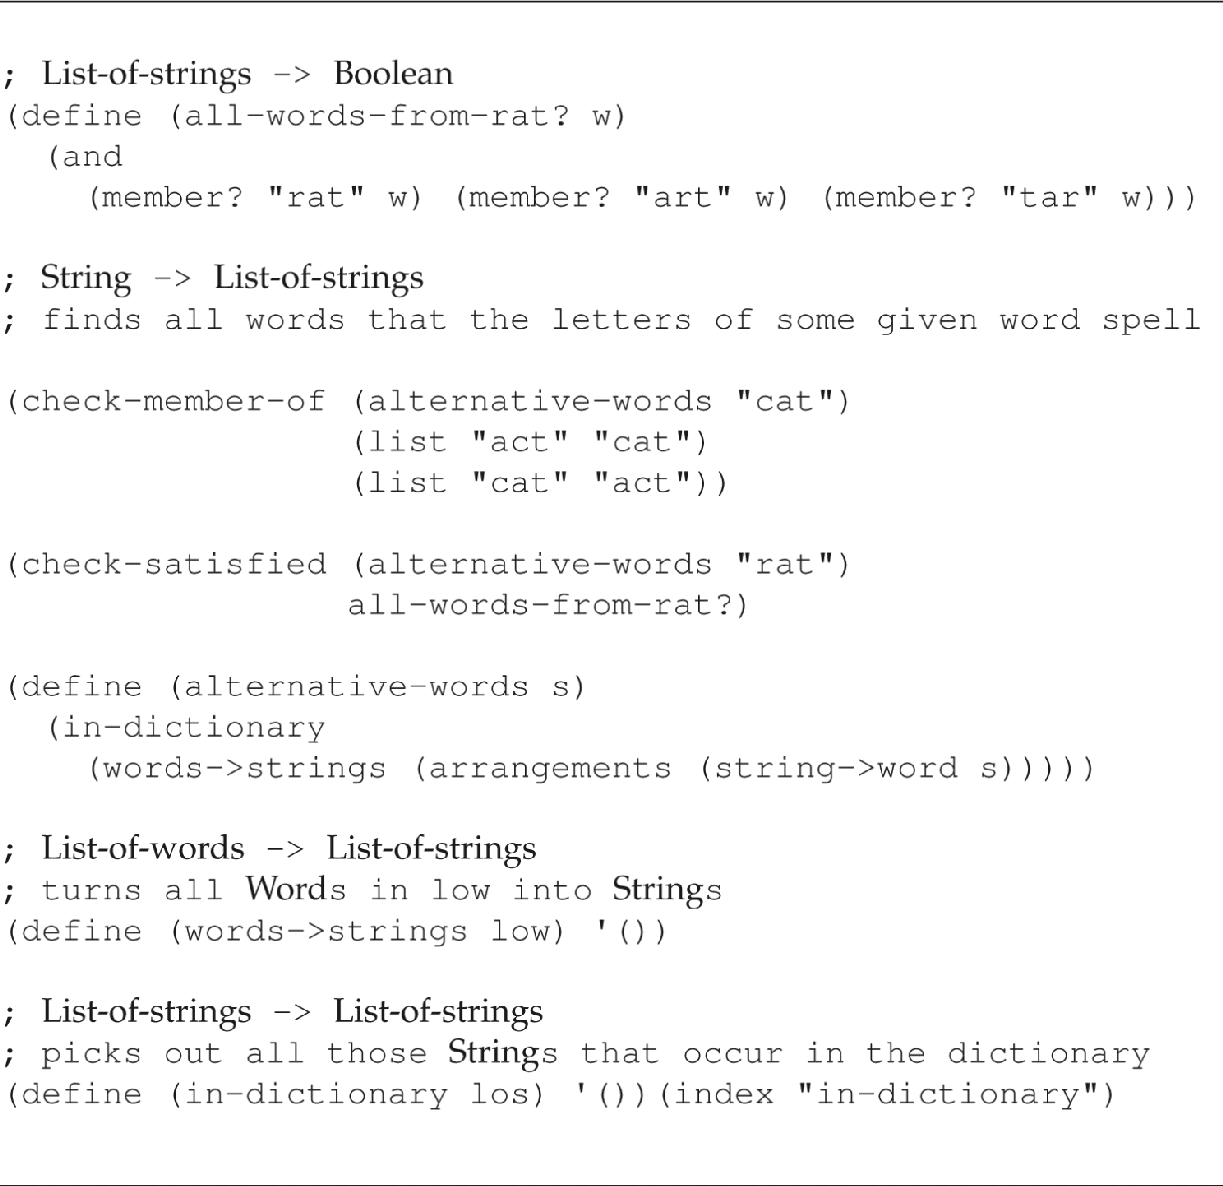
\includegraphics[width=0.85\textwidth]{images/00284.png}
  \caption{单词异序词查找程序的组合设计架构}
  \label{fig:finding_alternative_words}
\end{figure}

\begin{exercise}{字符串与单词表示的双向转换}{209}
为了便于递归重排字符，我们使用单字符列表 \code{Word} 表示单词：
\begin{lstlisting}[language=BSL]
; A Word 是以下之一：
; -- '()
; -- (cons 1String Word)
\end{lstlisting}
利用内置的 \code{explode} 与 \code{implode} 设计 \code{string->word} 与 \code{word->string}。
\end{exercise}

\begin{exercise}{单词列表批量转换为字符串列表 words->strings}{210}
设计函数 \code{words->strings}：消耗 \code{List-of-words} 并产生对应的 \code{List-of-strings}。
\end{exercise}

\begin{exercise}{词典有效性过滤 in-dictionary}{211}
设计函数 \code{in-dictionary}：消耗字符串列表，筛选并仅保留那些收录在系统词典中的合法单词。
\end{exercise}

\section{单词游戏：问题的核心}
\label{sec:ch12_word_games_heart}

本节解决整个字谜程序的核心与难点：设计函数 \code{arrangements}，计算一个 \code{Word} 的全排列（Permutations）。

\begin{exercise}{全排列数据定义与示例}{212}
写出 \code{List-of-words} 的自引用数据定义，并针对两字母单词（如 \code{"d"} 和 \code{"e"}）编写全排列的功能示例。
\end{exercise}

对于一个单词 \code{w}：
\begin{itemize}
  \item 若为空词 \code{'()}，其全排列仅有唯一一种可能：\code{(list '())}；
  \item 若为非空词，自然递归 \code{(arrangements (rest w))} 将求出剩余所有字符的全排列；
  \item 此时，主任务转化为：\textbf{如何将首字符 \code{(first w)} 插入到上述每个单词的所有可能缝隙中（开头、中间所有位置、末尾）}！
\end{itemize}

我们将这一新任务委托给辅助函数 \code{insert-everywhere/in-all-words}：
\begin{lstlisting}[language=BSL]
(define (arrangements w)
  (cond
    [(empty? w) (list '())]
    [else (insert-everywhere/in-all-words (first w)
                                          (arrangements (rest w)))]))
\end{lstlisting}

\begin{exercise}{全缝隙插入函数 insert-everywhere/in-all-words}{213}
设计函数 \code{insert-everywhere/in-all-words}：消耗单字符 1String 与单词列表，将该字符插入到每个单词的每一个可能位置（使用 \code{append} 拼接列表）。
\end{exercise}

\begin{exercise}{联调集成与端到端运行}{214}
将 \code{arrangements} 与 12.3 节的模块整合，运行全套测试，并在真实词汇上进行字谜求解实验。
\end{exercise}

\section{喂贪吃蛇}
\label{sec:ch12_feeding_worms}

贪吃蛇（Worm / Snake）是经典的街机游戏：蛇在屏幕中移动，玩家通过方向键改变其前进方向；每吃到一个食物，蛇身增长一节并获得分数；若蛇头触碰边界或咬到自身躯干，游戏即告结束（如图~\ref{fig:playing_worm} 所示）。

\begin{figure}[htbp]
  \centering
  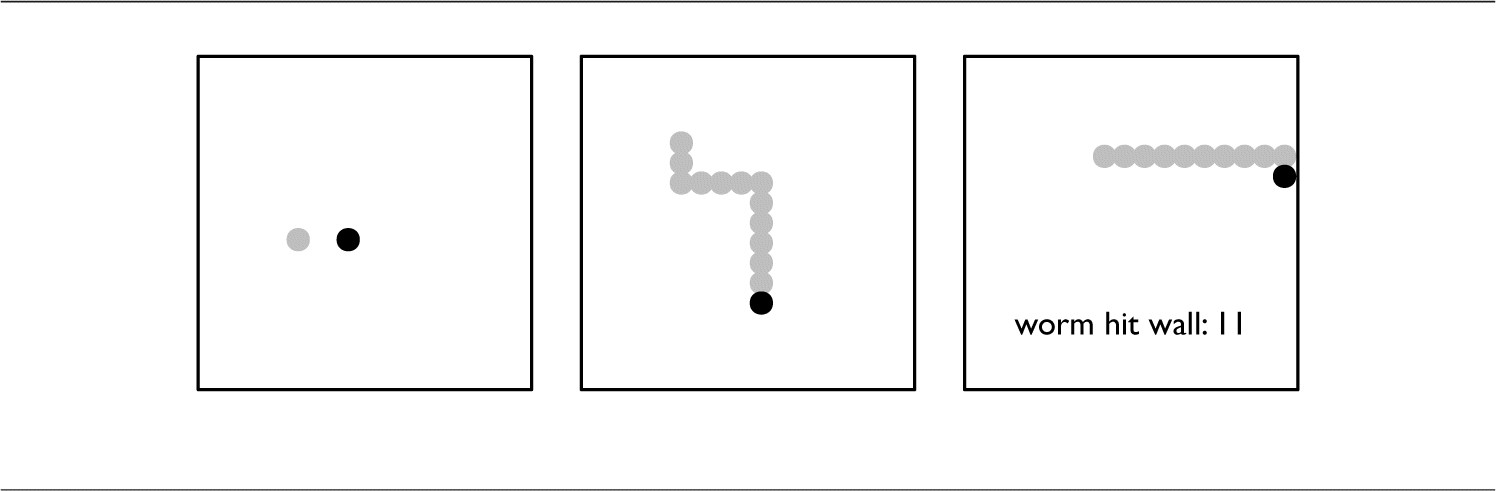
\includegraphics[width=0.85\textwidth]{images/00289.png}
  \caption{贪吃蛇游戏截图}
  \label{fig:playing_worm}
\end{figure}

我们将通过迭代细化逐步构建整个游戏：

\begin{exercise}{第一阶段：单节蛇与方向控制}{215}
设计一个世界程序：蛇由单个红色圆盘（蛇头）构成，每个时钟节拍沿当前方向前进一个圆盘直径的距离，玩家可通过四个方向键改变行进方向。
\end{exercise}

\begin{exercise}{第二阶段：触壁死亡判定}{216}
为练习 215 的程序添加触壁检测：当蛇头触及画布边界时停止游戏，并在画面左下角渲染提示文本 \code{"worm hit border"}。
\end{exercise}

\begin{exercise}{第三阶段：多节蛇身游动}{217}
将蛇身的数据表示泛化为 \code{Posn} 列表（表头为蛇头，其余为按序跟随的躯干节点）。实现多节蛇身的平滑游动（提示：每次前进时在蛇头方向 \code{cons} 一个新节点，并切除尾部的最后一个节点）。
\end{exercise}

\begin{exercise}{第四阶段：自身碰撞检测}{218}
完善游戏结束规则：当蛇头与自身现存的任意躯干节点坐标重合时，判定游戏结束并显示撞击自身提示。
\end{exercise}

\begin{exercise}{第五阶段：投放食物与得分增长}{219}
引入随机放置的食物（如图~\ref{fig:random_food} 所示的生成逻辑）。当蛇头覆盖食物坐标时，吃掉食物并将身体延长一节，同时在随机位置刷新下一枚食物。
\end{exercise}

\begin{figure}[htbp]
  \centering
  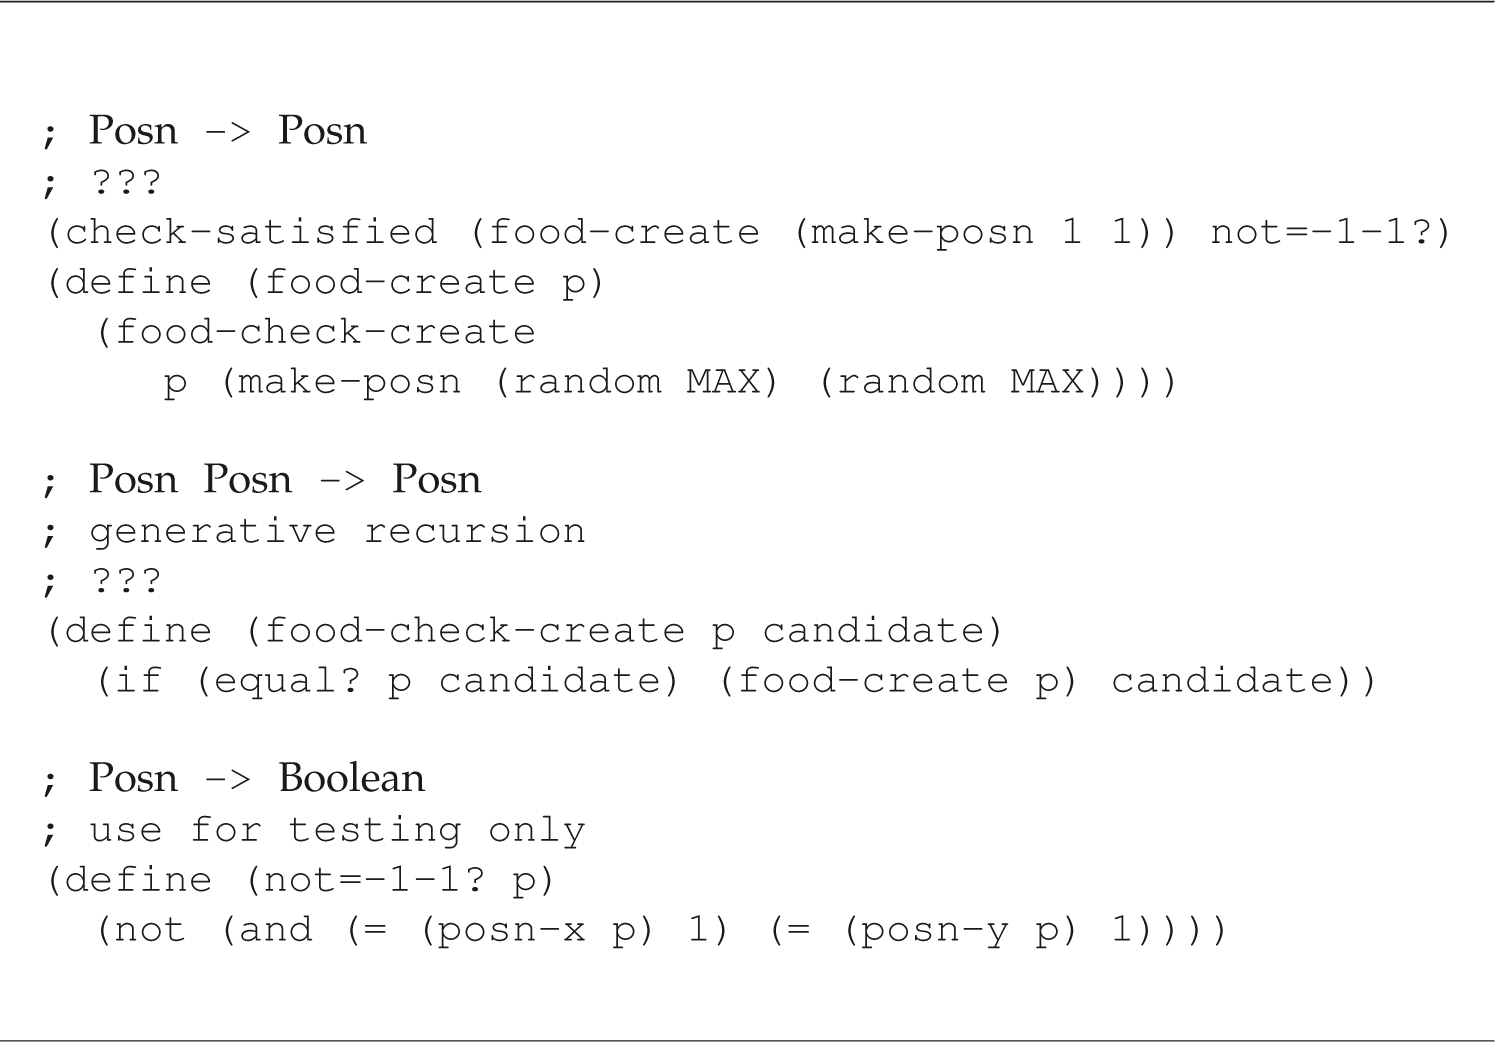
\includegraphics[width=0.85\textwidth]{images/00290.png}
  \caption{食物的随机坐标生成逻辑}
  \label{fig:random_food}
\end{figure}

\section{简易俄罗斯方块}
\label{sec:ch12_simple_tetris}

俄罗斯方块（Tetris）是另一款风靡全球的经典游戏。在此项目中，我们实现一个规则精炼的简易版本：单个方块从顶部缓慢坠落，玩家可通过左右方向键调整其下落列位置；一旦方块触底或叠落在已有方块之上，它便冻结在原地，随后顶部重新生成新的方块；当堆叠高度触及画布顶端时，游戏结束（如图~\ref{fig:simple_tetris} 所示）。

\begin{figure}[htbp]
  \centering
  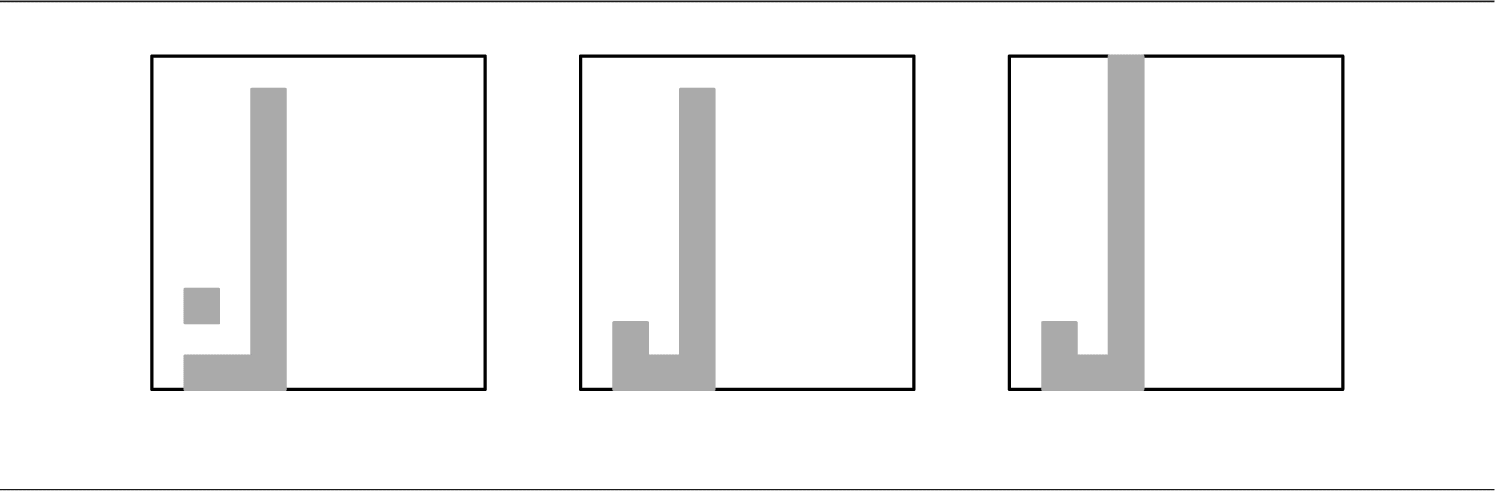
\includegraphics[width=0.75\textwidth]{images/00291.png}
  \caption{简易俄罗斯方块游戏示意图}
  \label{fig:simple_tetris}
\end{figure}

世界状态数据定义采用网格逻辑坐标：
\begin{lstlisting}[language=BSL]
(define-struct tetris [block landscape])
(define-struct block [x y])

; A Tetris 是一个结构体：(make-tetris Block Landscape)
; A Landscape（地貌列表）是以下之一：
; -- '()
; -- (cons Block Landscape)
; A Block 是一个结构体：(make-block N N)
; 解释：block 代表当前正在下落的方块；landscape 代表已经着陆堆叠的所有方块。
\end{lstlisting}

\begin{exercise}{渲染游戏场景 tetris-render}{220}
设计函数 \code{tetris-render}：将当前的 \code{Tetris} 状态（包含下落方块与静态地貌方块列表）绘制在网格画布上。
\end{exercise}

\begin{exercise}{下落与堆叠判定 tetris-main}{221}
编写时钟更新函数：方块垂直下落；当检测到方块触底或下移一步将与地貌中的某个方块重叠时，将当前方块冻结并转移入地貌列表，并生成一个新方块。
\end{exercise}

\begin{exercise}{水平移动控制}{222}
添加键盘事件处理：响应左右方向键移动下落方块，并防止方块穿透侧壁或嵌入侧边已有的方块堆中。
\end{exercise}

\begin{exercise}{顶格游戏结束判定}{223}
使用 \code{stop-when} 监听：当任何一列的方块堆叠触及顶部边界时终止游戏，并展示最终得分。
\end{exercise}

\section{完整的太空大战}
\label{sec:ch12_full_space_war}

\begin{exercise}{综合世界项目：太空入侵者}{224}
综合运用本章所学的多对象列表控制技术，将第 6 章的飞碟入侵防御游戏完善为全功能版：坦克可在地面自由移动，并可任意发射多枚导弹；飞碟以特定轨迹降落并可投掷炸弹；实现弹幕与飞碟的精准碰撞判定。
\end{exercise}

\begin{exercise}{创意设计：森林灭火飞行模拟}{225}
设计空中灭火游戏：模拟森林发生随机野火，玩家驾驶消防飞机水平巡航并适时投放水弹灭火，在限定时间内扑灭所有林火。
\end{exercise}

\section{有限状态机}
\label{sec:ch12_finite_state_machines}

\term{有限状态机}（Finite State Machines, FSM）是计算机科学的基石理论之一。在第 4.7 节中，我们曾通过硬编码的条件分支实现过交通信号灯。现在，我们能够设计一个通用的\term{状态机解释器}：它接受任意状态机的数据描述，并驱动其运行。

图~\ref{fig:general_fsm} 给出了通用的状态机数据定义与交互模拟模型。

\begin{figure}[htbp]
  \centering
  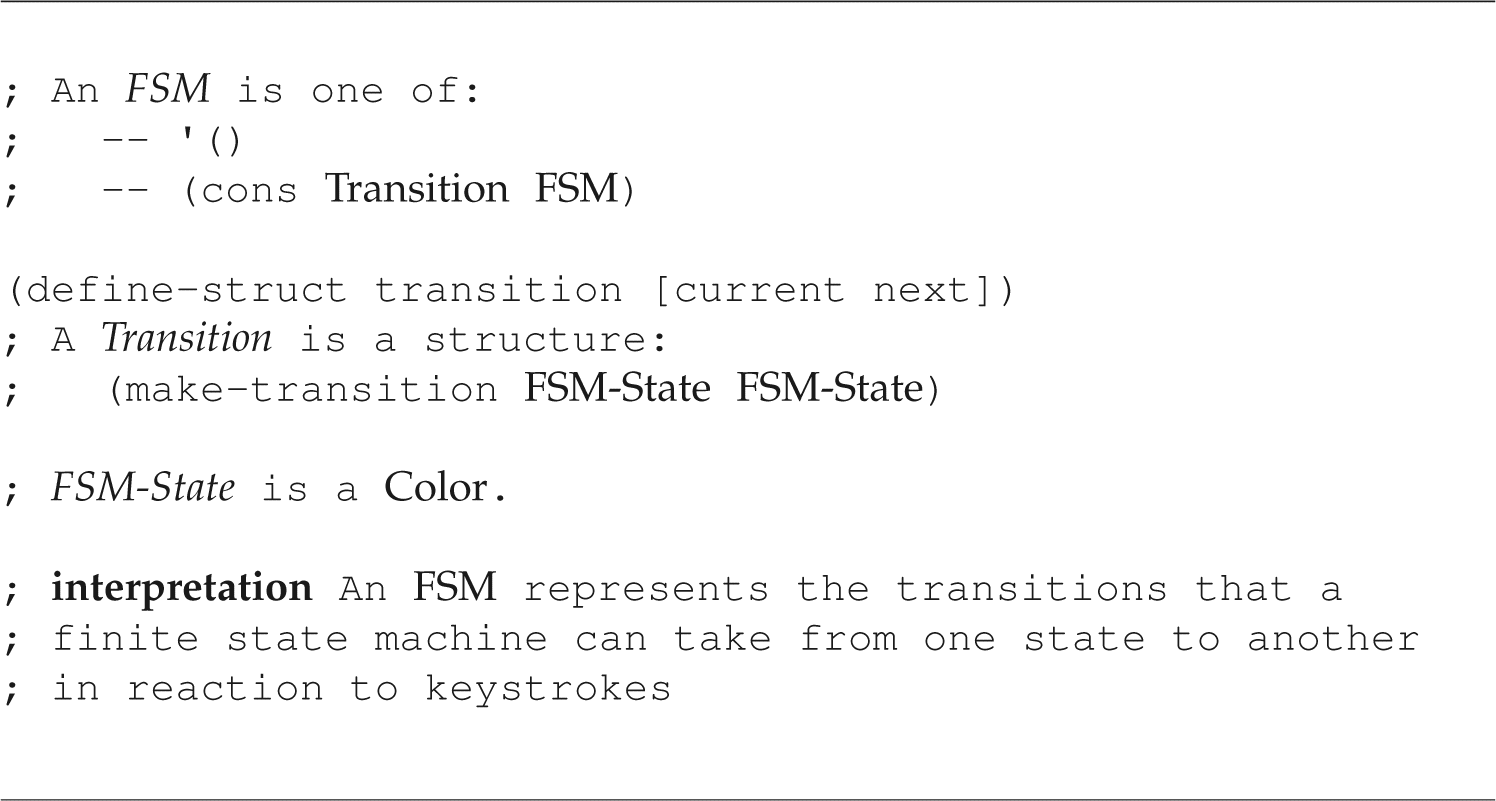
\includegraphics[width=0.85\textwidth]{images/00295.png}
  \caption{通用有限状态机的数据表示与模拟器框架}
  \label{fig:general_fsm}
\end{figure}

\begin{exercise}{状态判等谓词 state=?}{226}
设计谓词 \code{state=?}：判断两个状态是否相等。
\end{exercise}

\begin{exercise}{黑白跳变状态机 BW Machine}{227}
构造一个每按任意键就在黑白两色之间往复跳变的状态机数据实例。
\end{exercise}

\begin{exercise}{状态跳转查找函数 find}{228}
设计函数 \code{find}：在转移列表 \code{FSM} 中查找当前状态匹配的转移规则，并输出下一状态。
\end{exercise}

\begin{exercise}{按键驱动的状态转移 Transition.v2}{229}
扩展转移规则结构体为 \code{(make-ktransition current key next)}，使状态转移严格依赖玩家所按下的特定按键。
\end{exercise}

\begin{exercise}{带初始与终止状态的终极 FSM 解释器}{230}
设计完整版数据模型 \code{(make-fsm initial transitions final)}，并实现通用解释器 \code{fsm-simulate}：当状态机流转到达终止状态时，自动平稳退出。
\end{exercise}
